\begin{title}[\Large]
  Параграф 2.3
\end{title}

\begin{title}[\Large]
  Длина дуги кривой на поверхности. Первая квадратичная форма поверхности
\end{title}

\begin{define}[первой квадратичной формы]
  $\vec \varphi = \vec \varphi(u, \upsilon)$ регулярная поверхность
  $$
  \vec \varphi' = \vec \varphi_u u' + \vec \varphi_{\upsilon} \upsilon'
  $$
  $$
  |\vec \varphi'|^2 = (\vec \varphi', \vec \varphi') =
  (\vec \varphi_u u' + \vec \varphi_{\upsilon} \upsilon',
  \vec \varphi_u u' + \vec \varphi_{\upsilon} \upsilon') =
  $$
  $$
  = (\vec \varphi_u, \vec \varphi_u)u'^2 + 2(\vec \varphi_u,
  \vec \varphi_{\upsilon}') u' \upsilon' + \upsilon'^2 (\vec \varphi_{\upsilon},
  \vec \varphi_{\upsilon})
  $$
  $E = (\vec \varphi_u, \vec \varphi_u)$

  $F = (\vec \varphi_u, \vec \varphi_{\upsilon})$

  $G = (\vec \varphi_{\upsilon}, \vec \varphi_{\upsilon})$

  зависят только от поверхности но не от кривой.

  $|\vec \varphi'|^2 = E u'^2 + 2Fu'\upsilon' + G\upsilon'^2$ кривая задана в
  локальной системе координат.

  $ds^2 = Edu^2 + 2Fdud\upsilon + Gd\upsilon^2$ первая квадратичная форма
  поверхности в дифференциале.

  $ds^2 = Edu^2 + 2Fdud\upsilon + Gd\upsilon^2$ определяет поверхность
  однозначно.
\end{define}

\begin{block}[Свойства]
  1) $E,G > 0$

  \begin{proof}
    $$
    E = (\vec \varphi_u, \vec \varphi_u) = |\vec \varphi_u|^2 > 0
    $$
    $$
    G = (\vec \varphi_{\upsilon}, \vec \varphi_{\upsilon}) =
    |\vec \varphi_{\upsilon}|^2 > 0
    $$
    лнз значит не являются $\vec 0$
  \end{proof}

  2) первая квадратичная формула положительна определена

  \begin{proof}
    $$
    F = (\vec \varphi_u, \vec \varphi_{\upsilon}) = |\vec \varphi_u|
    |\vec \varphi_{\upsilon}| \cos \alpha
    $$
    $$
    \left|
    \begin{array}{cc}
      E & F \\
      F & G
    \end{array}
    \right|
    = EG - F^2 = |\vec \varphi_u|^2|\vec \varphi_{\upsilon}|^2 -
    |\vec \varphi_u|^2 |\vec \varphi_{\upsilon}|^2 \cos^2 \alpha =
    $$
    $$
    = |\vec \varphi_u|^2
    |\vec \varphi_{\upsilon}|^2 \sin^2 \alpha = |[\vec \varphi_u, \vec
    \varphi_{\upsilon}]|^2 > 0
    $$
    так как $\vec \varphi_u, \vec \varphi_{\upsilon}$ лнз из за регулярности
    поверхности $\Rightarrow ~ \not= \vec 0$
  \end{proof}
\end{block}

\begin{block}[Длина дуги на поверхности]
  $\vec \varphi = \vec \varphi(u, \upsilon)$ регулярная поверхность
  $$
  \left\{
    \begin{array}{l}
      u = u(t) \\
      \upsilon = \upsilon(t)
    \end{array}
  \right. ~ \text{кривая на поверхности, тогда} ~~
  s = \int_{t_0}^{t_1} |\vec \varphi'(t)| dt ~ \text{длина}
  $$
  $$
  s = \int_{t_0}^{t_1} \sqrt{E u'^2 + 2Fu'\upsilon' + G\upsilon'^2}dt
  $$
\end{block}

\begin{title}[\Large]
  Приложения первой квадратичной формы для вычисления скалярного произведения
  касательных векторов, угла между кривыми, площади области поверхности
\end{title}

\begin{block}[Вычисление скалярного произведения касательных векторов]
  $$
  \vec a = \xi_1 \vec \varphi_u + \xi_2 \vec \varphi_{\upsilon} ~~~
  \vec b = \zeta_1 \vec \varphi_u + \zeta_2 \vec \varphi_{\upsilon}
  $$
  $$
  (\vec a, \vec b) = (\xi_1 \vec \varphi_u + \xi_2 \vec \varphi_{\upsilon},
  \zeta_1 \vec \varphi_u + \zeta_2 \vec \varphi_{\upsilon}) =
  E \xi_1 \zeta_1 + F(\xi_1 \zeta_2 + \xi_2 \zeta_1) + G\xi_2 \zeta_2
  $$
  $$
  |\vec a| = \sqrt{(\vec a, \vec a)} = \sqrt{E\xi_1^2 + 2F\xi_1 \xi_2 +
  G\xi_2^2}
  $$
\end{block}

\begin{block}[Угл между кривыми]
  $$
  \vec a = \xi_1 \vec \varphi_u + \xi_2 \vec \varphi_{\upsilon} ~~~
  \vec b = \zeta_1 \vec \varphi_u + \zeta_2 \vec \varphi_{\upsilon}
  $$
  $$
  \cos \measuredangle (\vec a, \vec b) =
  \frac{(\vec a, \vec b)}{|\vec a||\vec b|} =
  \frac{E \xi_1 \zeta_1 + F(\xi_1 \zeta_2 + \xi_2 \zeta_1) + G\xi_2 \zeta_2}
  {\sqrt{E\xi_1^2 + 2F\xi_1\xi_2 + G\xi_2^2}
  \sqrt{E\zeta_1^2 + 2F\zeta_1\zeta_2 + G\zeta_2^2}}
  $$
  Расмотрим следующие кривые
  $$
  \vec \varphi_1 =
  \left\{
    \begin{array}{l}
      u = u_1(t) \\
      \upsilon = \upsilon_1(t)
    \end{array}
  \right. ~~~
  \vec \varphi_2 =
  \left\{
    \begin{array}{l}
      u = u_2(t) \\
      \upsilon = \upsilon_2(t)
    \end{array}
  \right.
  $$
  Угол между кривыми это угол между их касательными в точке пересечения

  $\cos \alpha = |\cos \measuredangle (\vec \varphi_1', \vec \varphi_2')|$

  $\vec \varphi_1' = \vec \varphi_u u_1' + \vec \varphi_{\upsilon}'
  \upsilon_1' = (u_1', \upsilon_1')$

  $\vec \varphi_2' = \vec \varphi_u u_2' + \vec \varphi_{\upsilon}'
  \upsilon_2' = (u_2', \upsilon_2')$
  $$
  \cos \alpha = \frac{Eu'_1 \upsilon'_1 + F(u'_1\upsilon_2' + u'_2 \upsilon'_1)
  + Gu_2' \upsilon'_2}
  {\sqrt{Eu_1'^2 + 2Fu_1'u_2' + Gu_2'^2}
  \sqrt{E\upsilon_1'^2 + 2F\upsilon_1'\upsilon_2' + G\upsilon_2'^2}}
  $$
\end{block}

\begin{block}[Площадь области поверхности]
  $d\upsilon = |[\vec \varphi_u du, \vec \varphi_{\upsilon} d\upsilon]| =
  |[\vec \varphi_u, \vec \varphi_{\upsilon}]| du d\upsilon$
  $$
  \theta = \iint \limits_{\Omega} |[\vec \varphi_u, \vec \varphi_{\upsilon}]|
  du d\upsilon = \iint \limits_{\Omega} \sqrt{EG - F^2}dud\upsilon
  $$
\end{block}

\begin{title}[\Large]
  Изометрические и конформные отображения поверхности. Стереографическая
  проекция
\end{title}

\begin{define}[изометрического отображения поверхности]
  Отображение поверхноси сохраняющая длины кривых и углы между кривыми
  называется изометрическим.
\end{define}

\begin{theorem}
  Поверхности локально изометричны $\Leftrightarrow$ можно выбрать
  параметризацию так что соответствующие первые квадратичные формы будут
  одинаковы.
\end{theorem}

\begin{define}[конформного отображения поверхности]
  Отображения поверхности сохраняющая углы между кривыми называется
  конформным.
\end{define}

\begin{theorem}
  Поверхности локально комфорны $\Leftrightarrow$ можно выбрать
  параметризацию так что соответсвующие первые квадратичные формы будут
  прапорцианальными.
\end{theorem}

\begin{define}[стереографической проэкции]
  Плоскость $N$ (северный полюс сферы) является точкой на максимальном
  расстоянии от плоскости $\Pi$. Через каждую точку $x \not= N$ сферы проходит
  единственная прямая $D$, соедининяющая $x$ и $N$. Прямая $D$ пересекает
  плоскость в единственной точке $X$, которая, таким образом, является образом
  точки $x$ при стереографической проекции. В результате получается взаимно
  однозначное отображение сферы с выколотой точкой $N$ на плоскость $\Pi$.

  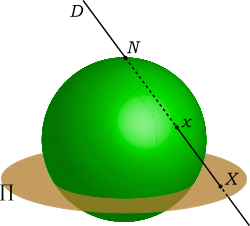
\includegraphics[width = 5cm]{StereoProjection}
\end{define}
